\documentclass[12pt,a4paper]{article}
\usepackage{times}
\usepackage{durhampaper}

\usepackage{harvard}
% package to add dumptext
\usepackage[english]{babel}
\usepackage{blindtext}

% package to add wrapfigure
\usepackage{wrapfig}

% packages to add images
\usepackage{graphicx}

% packages for pseudocode and algorithms
\usepackage{amsmath}
\usepackage{algorithm}
\usepackage[noend]{algpseudocode}
\makeatletter
\def\BState{\State\hskip-\ALG@thistlm}
\makeatother

% packages to generate neural network graph
\usepackage{tikz}
\usetikzlibrary{matrix,chains,positioning,decorations.pathreplacing,arrows}


% package to add graphs
\usepackage{pgfplots}

\citationmode{abbr}
\bibliographystyle{agsm}

\title{Improving CNN Draughts Evaluators using Genetic Algorithms}
\author{Thien P. Nguyen}
\student{Thien P. Nguyen}
\supervisor{Stefan Dantchev}
\degree{BSc Computer Science}

% stuff for checkerboard
\usetikzlibrary{matrix.skeleton}
\tikzstyle{ball} = [circle, shading=ball, minimum size=1cm]
\newcommand{\bl}{\node [ball, ball color=black!80!white, draw=black!65!white, thin]{};}
\newcommand{\wh}{\node [ball, ball color=white] {};}


% -------------------------------------------------------------------

\begin{document}

\maketitle

\begin{abstract}

    {\bf Background}

    Presently, competitive Draughts AI players are currently designed to play at a fixed ability. While it has produced very competitive and intelligent players, they require manual modifications in order to improve its performance. This is due to their dependency on pre-defined move databases, where optimal moves are pre-calculated, and recalled when necessary. By combining Neural Networks and Genetic Algorithms, this issue could possibly be solved by creating a player that can grow in ability over time, without the dependency on move-banks.
    
    {\bf Aims}

    The purpose of this project is to explore approaches to tackle the game of English Draughts via the use of  machine learning techniques. First, we study previous historical successes in the field, and look at the components that helped build their systems. Then, we look at contemporary methods of computer science that could be used to evolve the historical systems. The project will establish whether this approach provides an effective performance on the game.
    
    {\bf Method}

    The initial population will consist of randomly generated AI players, which will play each other to determine the best player out of the population. The performance of championing AI players at every generation of the genetic algorithm are measured against previous champions. Appropiate algorithms are implemented to detect the overall development of the system's ability to play Checkers.

    {\bf Proposed Solution}.  

    The proposed solution starts with designing a neural network that evaluates the probability of a particular side winning, given a given state of a checkerboard. This is then used in a algorithm that evaluates future moves to predict the best move at a given position. This, alongside a set of weights for the neural network, creates a player that can evaluate potential moves. Finally, the player is then used on an existing Draughts framework that will provide the player with the ability to play Draughts.

\end{abstract}

\begin{keywords}
AI, Neural Networks, Genetic Algorithms, MiniMax, Alpha Beta Pruning, Draughts

\end{keywords}

% ----------------

% Sort introduction to your project
% This will be the first thing that your second marker sees about your project
% Make sure they can understand what you’re doing
% Write for educated reader with background in CS, but non-expert Should contain:

%   Brief introduction to the project
%   The research question you are addressing
%   Aims of the project 
%   Deliverables


\section{Introduction}

    The intention of this project is to explore the effectiveness of genetic algorithms to improve the evaluation of a neural network. Neural networks are used to determine the performance of two players in a game of checkers. We attempt to use various crossover and mutation strategies to manipulate the neurons of the network in order to increase the accuracy of the measurements. This would allow us to create an effective Draughts playing agent that would have the ability to learn without human input.

\subsection*{Draughts}

    English Draughts (or Checkers) is a popular 2-player boardgame played on an 8x8 chessboard. Players begin with 12 pieces each, and they are placed on light-coloured squares. Each player takes a turn to move a piece diagonally in one square. They also have the option to capture their opponments piece by moving two consecutive diagonal squares, where the opponments piece is placed immediately opposite the players piece. Pieces can be captured consecutively in a single turn if the moves afford the scenario. In the event that a piece reaches the opposite side of the board from where the piece started with, they are promoted to a King piece. King pieces have the ability to traverse backwards in the same diagonal motion as pawns. A player wins by capturing all of their opponments pieces. A player loses by having all of their pieces captured. A draw occurs when there is both players agree to draw after a  three-fold repetition, or a player has pieces on the board but cannot move any of them.

\subsection*{Genetic Algorithms}

    Genetic algorithms (GAs) are a group of search techniques used to find exact or approximate solutions to optimisation and search problems. It borrows techniques from Charles Darwin's evolutionism theory; individuals are created by the crossover of the genetic information of their parents. 
    Genetic algorithms are a subset of evolutionary algorithms, which is also formed of similar strategies, which also include evolutionary programming [Fogel, 1993][McDonnel, 1993], and genetic programming [Koza, 1991]. Genetic Algorithms focus on the use of genome manipulation via the use of crossover algorithms and mutation methods. Genomes are a metaphor of genetic information, where it typically refers to an 1D array.

\subsection*{Neural Networks}

    Neural Networks are non-linear statistical data-modelling tools, linking inputs and outputs adaptively in a learning process similar to how the human brain operates. Networks consist of units, described as neurons, joined by a set of rules and weights. The units are defined with characterisitics, and appear in layers. The first layer is defined as the input layer, and the last layer being the output. Layers between the two aforementioned are described as hidden layers. Data is analysed by processing them through the layers.

    Learning takes place in the form of the manipulation of the weights connecting the units in the layers. This allows it to model complex relationships between inputs and output, and it can also find patterns in the data. 

\subsection*{Motivation}
    % Research Question
    Whilst the use of evolutionary algorithms and neural networks have been explored to create draughts players, my intention is to explore the effectiveness of genetic algorithms. My intention is to determine whether it is possible to  produce a performant draughts playing agent by the use of GANNs (Genetic Algorithms and Neural Networks). 

\subsection*{Deliverables}

    \subsubsection*{Minimum}

    \begin{itemize}
    \item Implement a CNN
    \item Implement a Checkers Game Interface
    \item Implement a genetic algorithm with an evaluation function that
    consists of a round robin tournament against the population of CNN
    Evaluators.
    \item Implement a mini-max algorithm that chooses moves.
    \end{itemize}

    \subsubsection*{Intermediate}

    \begin{itemize}
    \item A user-friendly interface to play against the AI
    \item A monte-carlo search of the move space.
    \item Analysis of Crossover methods (within Genetic Algorithms)
    \item Analysis of Mutation methods (within Genetic Algorithms)
    \end{itemize}

    \subsubsection*{Advanced}

    \begin{itemize}
    \item Convolutional Neural Network Layer analysis
    \item The resulting AI can play to an ELO of at least 1200.
    \end{itemize}

\subsection*{Related Work}

    Arthur Samuel in the 60's pioneered the concept of AI that can play Checkers, through the proposal of using genetic algorithms to produce a Draughts playing agent \cite{samuel_studies_2000}. However, the work described did not consider the use of neural networks (as it was not conceived at the time). Also, it was dependent on a set of heuristics that he devised, which caps the agent's ability to play to the effectiveness of Samuel's heuristics. 

    The idea of evolving neural networks to play Draughts is based on the success Chellapilla and Fogel had in evolving their own Checkers neural networks using far less sophisticated hardware \cite{chellapilla_evolving_1999}. Their work, Blondie24, used a neural network as the evaluator function, and used an evolutionary algorithm to evolve the agents. However, new agents are made strictly through the use of mutation. Blondie24's neural network structure consists of a $\left\{ 32,40,10,1 \right\}$ set. Spatial awareness as it takes an immediate input of the positions on the board. This makes it inherently more difficult for the neural network to generate heuristics based on spatial awareness as it is not immediately considered.

% ----------------

\section{Design}

\subsection*{Requirements}

    % Functional Requirements
    \subsubsection*{Functional Requirements}


    \begin{center}
        \begin{tabular}{| l  | l | l |}
        \hline
        Code & Description & Priority \\ \hline
        F1 & A checkers gameboard is created.& High  \\ \hline
        F2 &  Agents are able to harness neural networks to assist in their move decision.& High  \\ \hline
        F3 &  Offspring agents can be created using parents. & High \\ \hline
        F4 &  The weights and biases of the Agent's neural network are saved to storage.& High  \\ \hline
        F5 &  Humans are able to play against the Agents. & High \\ \hline
        \end{tabular}
    \end{center}


    % Non Functional Requirements
    \subsubsection*{Non-Functional Requirements}

        
    \begin{center}
        \begin{tabular*}{1\textwidth}{| l | p{144.5mm} |}
        \hline
        Code & Description \\ \hline
        N1 & Agents only choose valid, legal moves. \\ \hline
        N2 & Agents always return a valid, legal move.\\ \hline
        N3 & Agents are able to play against other agents. \\ \hline
        \end{tabular*}
    \end{center}


    % Table 1 shows the functional requirements identified for the program(s) that will be required for the project. FR-1 through FR-6 are handled by the server and player implementations in the GGP-Base package. FR-7 will require some modification to the server code in order to output the informationthatwillbeusedintheanalysisanddiscussionoftestingresults.
    % Table 2 shows the non-functional requirements that arise from the rules that will be applied for testing. Any failure of the agent to return a move through either error or timeout should be con- sidered a failure as per the AAAI GGP competition rules. The moves returned should always be valid and legal for the current state of the game. Since agents are given a fixed time period to choose a move, with no penalty or bonus applied so long as the move is returned within the allot- ted time, it makes sense that agents should be designed in such a way as to make best use of the time they are given.
    % The GGP-Base package addresses a number of these requirements and a number of test-games will be played to ensure they are adequately satisfied and the package functions as expected.

\subsection*{Algorithms and Data Structures}

\subsubsection{MiniMax Decision Making}

    In order to choose the best move given a current position, the decision making process for an agent revolves around the use of minimax algorithm. This algorithm expands the tree of potential moves until some depth is reached. at a given depth, an evaluation function is used to calculate the value of the given move. Best moves in a given set become their parents value. These values propagate upwards to the children of the root node. The use of alpha-beta pruning will help to prune unnecessary moves,  reducing the number of calculations. From here, the best child node is chosen, which represents the best move to make.

    The mini-max method will have a search depth of 4ply (where the agent will search two moves ahead.) This will allow the agents to have a basic stategy where they can plan their moves in advance. Theere are inherent tradeoffs with having a higher ply count; where the asymptopic complexity is expoential; it being $O(x^y)$ with $x$ being the branching factor, and y being the depth. The branching factor will consist of the moves from each agent in a given game. This expotential growth is the achillies heel to the mini-max approach. Evaluation functions may be difficult to obtain, especially in the case for Checkers, where branching factors can be very large. 

    Once the initial system is ready, we can migrate to a hybrid technique that combines Mini-max and Monte-Carlo Tree Search (called MCTS-EPT or MCTS with early playout termination) introduced by Lorentz \cite{lorentz_using_2016}. Monte-Carlo Tree search differs from mini-max where future moves are randomly played to the end of the game. It acts as a sampling of possible outcomes, and does not depend on an evaluation function at all. The random simulation of games are skewed such that more reasonable moves are chosen. MCTS-EPT modifies the random playout approach from traditional MCTS. Instead of allowing the random moves play to the end of the game, the number of moves traversed are capped and an evaluation function can be used from that caped position instead. The termination ply would be capped at 6ply.
    
    \begin{figure}[ht!]
        \centering
        \caption{The chosen neural network model. Note that the checkboard is preprocessed. \label{overflow}}
        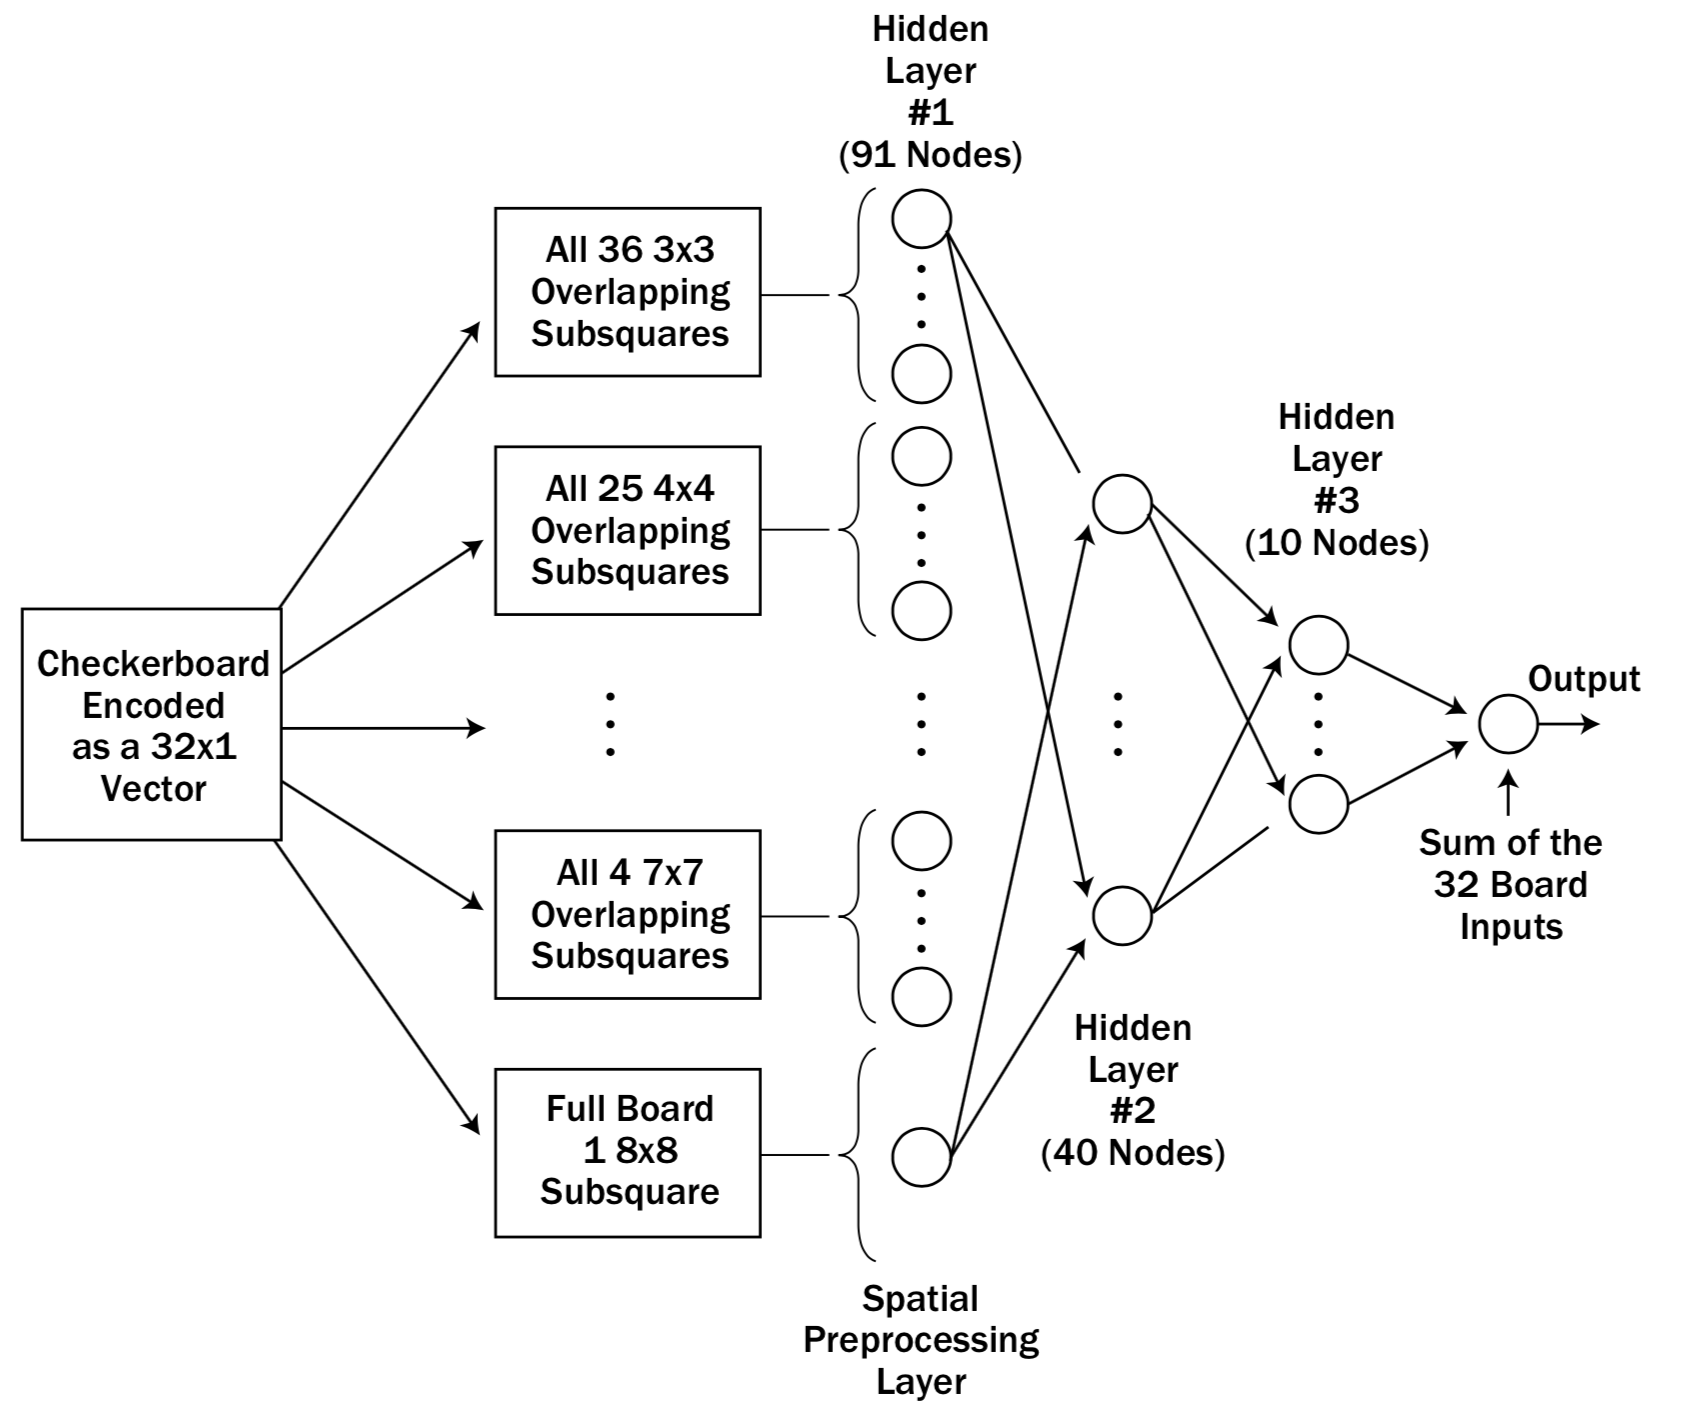
\includegraphics[width=60mm]{nnmodel.png}
    \end{figure}

    
\subsubsection{Neural Network}


    \begin{wrapfigure}{l}{0.37 \textwidth}
        % \begin{center}
        \vspace{-25pt}
        \centering
            \caption{The indexes of the 32 pieces of the input layer are the immediate values of the positions on the board. \label{boardarray}}
            \vspace{5pt}
            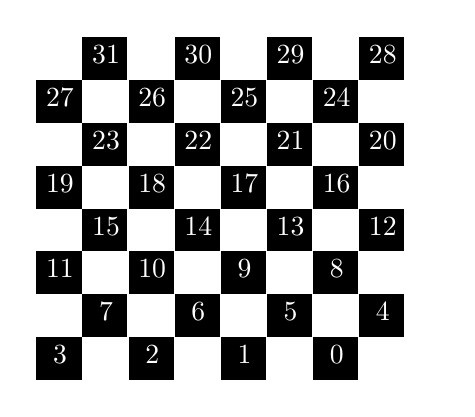
\begin{tikzpicture}
            \color{white}
            \matrix (m) [matrix of nodes, nodes in empty cells, label skeleton, nodes={minimum size = 0.4cm}] {
            & 31 &&30&&29&&28 \\
            27 &&26&&25&&24&&\\
            &23&&22&&21&&20\\   
                19&&18&&17&&16&&\\
            &15&&14&&13&&12\\
            11&&10&&9&&8&&\\
            &7&&6&&5&&4\\
            3&&2&&1&&0\\
            % \bl &     & \bl &     &     &     & \bl &     \\
            %     &     &     & \bl &     &     &     &     \\
            % \wh &     &     &     &     &     &     &     \\
            %     &     &     & \wh &     & \wh &     & \wh \\
            % \wh &     & \wh &     & \wh &     & \wh &     \\
            %     & \wh &     & \wh &     & \wh &     & \wh \\
            };
            \foreach \row in {1, ..., 8} {
            \foreach \col in {1, ..., 8} {
                \pgfmathparse{Mod(\row + \col, 2) ? "black" : "white"}
                \colorlet{squarebg}{\pgfmathresult}
                \fitandstyle[background]{(m-cell-\row-\col)}{fill = squarebg}
            }
            }
            \end{tikzpicture}
        % \end{center}
      
    \end{wrapfigure}


    In order to evaluate the board, we use a feed-forward multilayer perceptron style neural network. The network contains 4 layers, where the input layer consists of 91 nodes, with the output node having 1. The hidden layers have 40 and 10 nodes respectively. Our input array takes in the form of the grid array of the board. The intention is to weigh the Black pawns with a value of 1, and white pawns as -1. 
    
    It is common knowledge that a King piece is worth more than a pawn, but it is disputed about its precise value advantage. For the sake of completeness, a King's piece value is to be weighted at 1.5x the regular pawn value. 

    To create the input layer, we treat the checkboard into a 1D array, with the indexes displayed in figure \ref{boardarray}. The array is used to calculate all possible subsquares of the checkerboard, ranging from a 3x3 kernel to a 8x8. Each subsquare is summed up to create an input node. There are consequently 91 combinations of the subsquares, thus forming the input layer. 



    
    % Eventually, we will move to  ReLU (Rectified linear unit), proposed by Hinton. ReLU 

    % Most of time tanh is quickly converge than sigmoid and logistic function, and performs better accuracy [1]. However, recently rectified linear unit (ReLU) is proposed by Hinton [2] which shows ReLU train six times fast than tanh [3] to reach same training error. And you can refer to [4] to see what benefits ReLU provides.
    
    \begin{wrapfigure}{r}{0.3\textwidth}
        \centering
        \vspace{-30pt}
        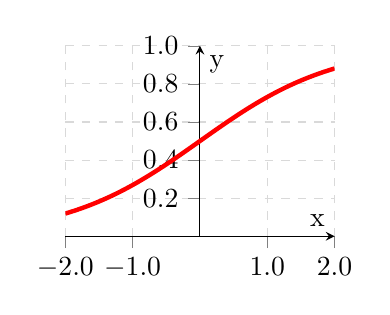
\begin{tikzpicture}
            \begin{axis}[
                legend pos=north west,
                axis x line=middle,
                axis y line=middle,
                x tick label style={/pgf/number format/fixed,
                                    /pgf/number format/fixed zerofill,
                                    /pgf/number format/precision=1},
                y tick label style={/pgf/number format/fixed,
                                    /pgf/number format/fixed zerofill,
                                    /pgf/number format/precision=1},
                grid = major,
                width=5cm,
                height=4cm,
                grid style={dashed, gray!30},
                xmin=-2,     % start the diagram at this x-coordinate
                xmax= 2,    % end   the diagram at this x-coordinate
                ymin= 0,     % start the diagram at this y-coordinate
                ymax= 1,   % end   the diagram at this y-coordinate
                %axis background/.style={fill=white},
                xlabel=x,
                ylabel=y,
                tick align=outside,
                enlargelimits=false]
            % plot the stirling-formulae
            \addplot[domain=-2:2, red, ultra thick,samples=500] {1/(1+e^-x))};
            % \addlegendentry{$f(x)=\frac{1}{1+e^{-5x}}$}
            \end{axis}
        \end{tikzpicture}
        \caption{graph of sigmoidal function $f(x)=\frac{1}{1+e^{-x}}$ \label{sigmoid}}
        \vspace{-30pt}
    \end{wrapfigure}
    
    Our initial choice for the activation function is the sigmoid function, shown in figure \ref{sigmoid}. There exists inherent issues related to the properties of their derivatives, discussed by Hinton. However, since this issue is related to the properties of a gradient based learning method and not through a stochastic learning method (which genetic algorithms are), this is not a concern for the project.

\subsubsection{Genetic Algorithms} 

    The genetic algorithm is the heart of the learning strategy of the system. Here we discuss the various algorithms that form the collection of GA stategies.

\subsubsection{Population Generation}

    The initial population will consist of randomly generated weights and biases of the neural network, with values from -1,1 inclusive. For a population size of 15, the next generation is created using the best five agents from the current generation. They will continue to play in the next generation. The agents are also chosen as a base to create 10 new agents from.

    The next eight players are generated through the use of crossover strategies. The weights of the 1st and 2nd place agents are used as input to the crossover strategy and will generate 4 offsprings. Two are reciprocal crossover representations from the crossover, and the other two being directly mutated from the parents themselves. Another four children will be created using the same strategy, with the 2nd and 3rd agent's weights.
    The remaining two will be direct mutations of the 4th and 5th place agents.

\subsubsection{Tournament Selection}

    The tournament selection process revolves around each agent in the population playing 5 games as Black, against randomly selected opponments. Each game lasts a maximum of 100 moves; if a winner is not deduced from the game after each player places 100 moves, then a draw is called. Draws are also called when there is a five-fold move repetition from both players. A win is worth $2$ points, a draw being none and a loss being $-1$ points. Both the agent and its opponment receives a score. Scores are tallied up at the end of the game. Players are sorted by the number of points they scored. The best players will have the highest number of points.

\subsubsection{Coefficent Mutation}

    Each weight of the neural network will be incremented by a random value that is created using the following formula, where $WeightP$ is the current weight, and $K$ represents the number of weights and biases in the neural network:

    $$ WeightN = WeightP + \frac{1}{\sqrt{2 * \sqrt{K} }}$$

    The weights, as explained earlier will have a hard cap of [-1, 1]. This would consequently mean that the mutation is not controlled, and dependent on the number of weights in the system; The more weights in the network implies a less significant mutation.

\subsubsection{Crossover Strategy}

    Two offsprings are created per a pair of parents, with each offspring being the reciprocal crossover of each other. The weights of both parents (now each treated as a 1D array of coefficents), are divided contingent on the number of weights and biases for a given layer. Each layer should be treated separately to reduce the potential dependency on a purely randomly generated neural network. For each set of weights in a given layer, the following algorithm represents the crossover process:

    % for each layer's weights:
    %     n = number of weights and biases in a given layer
    %     index1 = random integer[0 to n]
    %     index2 = random integer[0 to n]
    %     if index2 < index1:
    %         swap index1 and index2's values
    %     Weights(child1) = $parent_{1}$[0 to index1] +  $parent_{2}$[index1 to index 2] + $parent_{1}$[index2 to n]
    %     Weights(child2) =  $parent_{2}$[0 to index1] + $parent_{1}$[index1 to index 2] +  $parent_{2}$[index2 to n]
        

    % add pseudocode here
    \begin{algorithm}
        \caption{Crossover Strategy}
        \begin{algorithmic}[1]
        \Procedure{crossover}{$parent_{1}$, $parent_{2}$}
        \BState \emph{loop} \text{for weights } $w$ \text{ in layers}:
        \State $n \gets \text{length of } w$
        % \State $\textit{stringlen} \gets \text{length of } \textit{string}$
        \State $i_{1} \gets \textit{random integer} (0,n-1)$
        \State $i_{2} \gets \textit{random integer} (0,n-1)$
        % \State $i \gets \textit{patlen}$
        % if statement to check random numbers
        \If {$i_{1} > i_{2}$}
        \State \textit{swap } $i_{1}$ \text{ and } $i_{2}$ 
        \EndIf
        % \State $j \gets \textit{patlen}$

        \State $weights_{w,child1}$ = $parent_{1}$[0 \ldots $i_{1}$] +  $parent_{2}$[$i_{1}+1$ \ldots $i_{2}$] + $parent_{1}$[$i_{2}+1$ \ldots $n$] 
        \State $weights_{w,child2}$ =  $parent_{2}$[0 \ldots $i_{1}$] + $parent_{1}$[$i_{1}+1$ \ldots $i_{2}$] +  $parent_{2}$[$i_{2}+1$ \ldots $n$] 
        
        \BState \textbf{Return} \emph{child1,child2}

        % \BState \emph{loop}:
        % \If {$\textit{string}(i) = \textit{path}(j)$}
        % \State $j \gets j-1$.
        % \State $i \gets i-1$.
        % \State \textbf{goto} \emph{loop}.
        % \State \textbf{close};
        % \EndIf
        % \State $i \gets i+\max(\textit{delta}_1(\textit{string}(i)),\textit{delta}_2(j))$.
        % \State \textbf{goto} \emph{top}.
        \EndProcedure
        \end{algorithmic}
    \end{algorithm}


\subsection*{Choice of Programming Language}

    There are several contenders, with each having their inherent benefits. C++ is a notable choice due to it's relatively lower level architecture, support for popular machine learning packages (most notably Google's TensorFlow.) In terns of performance, C++ trumps most languages. C++ has notable parallelised packages, (A popular library is OpenMP) which can assist in the overall performance of the system. However, it would be difficult to write, due to my unfimiliarity with the language. Also, programs written in this language are less portable. It is not suitable for running on university machines without the use of a sandbox. Improperly handled bugs can cause a fatal error on university machines.

    Javascript is a contender; Node.JS is a very powerful and popular package manager, $npm$. It is difficult to write multi-processed programs as Node.JS runs on a single thread by nature. It also lacks the support of popular machine learning libraries and performs relatively slower in some programming operations.

    I have chosen Python 3.6 due to my familiarity, and the support of popular scientific packages including NumPy and other machine learning tools. Python is also portable with a very wide compatability; for instance it is pre-installed on all popular UNIX machines and also has support from the university machines. Python development will be on Visual Studio Code, which again is a familiar tool and is also suited to the project.

    Object Oriented approaches are taken for the majority of the components of the system, ranging from the neural network library to the tournament system. Data structures are implemented using their own classes and methods where applicable. The modularity of object oriented programming provides the afforance of easier debugging and testing.

    Players weights (for their neural networks) are stored in two forms, one of which is to be stored on an MongoDB NoSQL instance, and another local copy in JSON. This allows the individual agents to be played against humans.

\subsection*{Tools}

    Initial runs will operate on a 1-ply load in order to determine the stability of the system on a 4-core Intel i5 6200u with 12GB's of memory. Development and debugging will occcur on this machine. Once testing has proven to be stable and lacking in errors, the system would run on Durham's MIRA (128-core Intel) distributed system with a 6-ply heavy load. In order to keep simulations running on MIRA, MOSH is used to maintain a consistent  connection to MIRA. The end champion is then transferred to the initial machine in order to be played against by human input.

\subsection*{Interface}

    \begin{wrapfigure}{r}{0.3\textwidth}
    % \begin{figure}[ht!]
        \vspace{-30pt}
        \centering
        \caption{An example CLI interface demonstrating a game of draughts between user input and an Agent. \label{cli_humaninput}}
        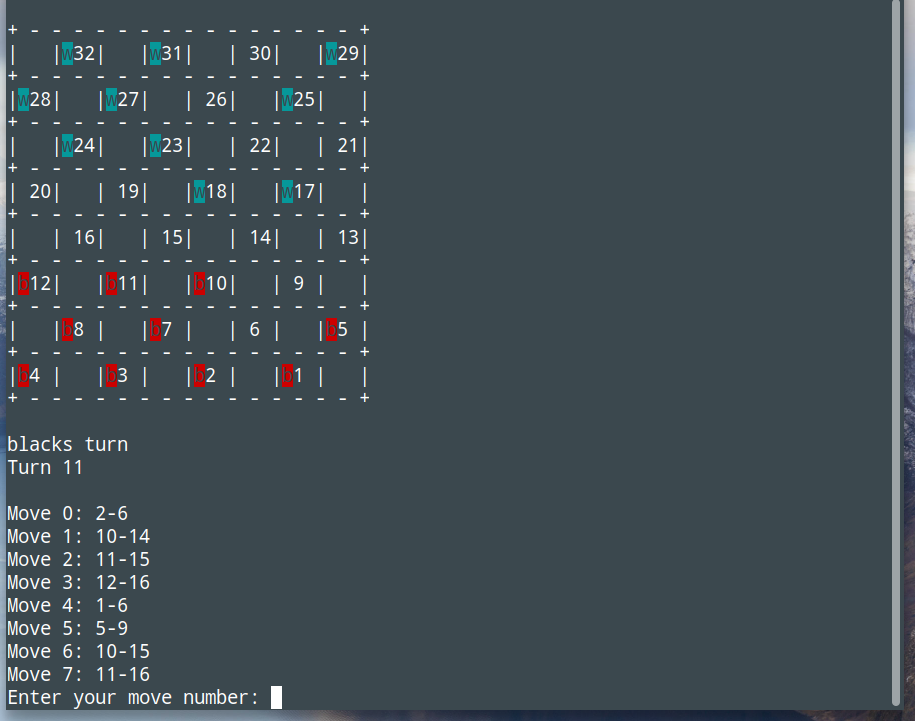
\includegraphics[width=43mm]{cli_humanvsagent.png}
        \vspace{-20pt}
    \end{wrapfigure}

    As our intention is to find an agent that plays Draughts, having a relatively friendly user interface is not necessarily important, i.e. a simple text-based interface will suffice. Due to the inherent computational strain the project requires, an interface based around having a command-line interface (CLI) the system is used. This allows the system to be initiated relatively faster than loading GUIs (Graphical User Interfaces), without the need for package dependencies, configurations and set-ups. It also reduces the amount of processing needed to render the most relevant statistics related to the project. The simulation would show information such as estimated finishing times, current generation count, scores of players in a given generation and the cummulative score of progress of the system.

    When it comes to humans playing against the agent, the checkerboard can also be rendered using ASCII plaintext, users can make inputs through text (in the console or terminal); where the game will show human users the possible moves that a person can take. This system will be used to play against the agent, where the human will take inputs the moves on behalf of the agent's online opponment. A possible rendition is shown in figure \ref{cli_humaninput}.

\subsection*{Testing and Evaluation}

    The combined GANN (Genetic Algorithm/Neural Networks) are evaluated under competition style conditions. At each generation, each agent plays 5 games, with their opponment being from randomly chosen from the generation pool. Point scores are measured by {2,0,-1} where 2 is a win, 0 is a draw, and -1 is a loss. There is a hard cap of 50 moves, where the game is considered a draw if after the game hasn't ended after 50 moves from each player.

    At the end of a given generation, we measure growth of performance using the champion of the generation. Presently we will use the mean of means approach. When a new chapmion is generated, it is played against the previous 5 champions from earlier generations. 6 games are played for each previous champion, with 3 being as Black, and 3 being White. A mean score is calculated from those 6 games. The overall performance of the current chapmion is the mean of the 5 sets of games. A positive improvement is when the mean of means are greater than 0. 

    Point Score for the champion games are measured by {1,0,-1} where a Win counts as 1 point and -1 for a loss. The weights are scaled differently to the regular tournament in order to accurately portray the difference between previous champions.

    At the end of the generation run, the end player will be used to compete against human players on various online multiplayers checkers websites in order to determine an accurate ELO rating of the system.


    % --------------------------------

% Presents the proposed solution(s)
% The design details should all be placed in this section
% Create a number of subsections, each focusing on one issue
% - Make it as clear as possible what you are planning to do
% - But not as a list of steps

% Writing skills (10%)
% • Clarity of presentation of ideas
% • Conformance to paper format standards as specified in Paper Template
% • Quality of writing(readability, grammar)
% • References

% Mark Scheme
% • Adequacy of the proposed solution
% • Specification and design
% • Identification of requirements
% • Description of tools used
% • Overview of architecture
% • Description of lifecycle

% ----------------
% Add references

\bibliography{zotero}

% The list of cited references should appear at the end of the report, ordered alphabetically by the surnames of the first authors.  The default style for references cited in the main text is the  Harvard (author, date) format.  When citing a section in a book, please give the relevant page numbers, as in \cite[p293]{budgen}.  When citing, where there are either one or two authors, use the names, but if there are more than two, give the first one and use ``et al.'' as in  , except where this would be ambiguous, in which case use all author names.

% You need to give all authors' names in each reference.  Do not use ``et al.'' unless there are more than five authors.  Papers that have not been published should be cited as ``unpublished'' \cite{euther}.  Papers that have been submitted or accepted for publication should be cited as ``submitted for publication'' as in \cite{futher} .  You can also cite using just the year when the author's name appears in the text, as in ``but according to Futher \citeyear{futher}, we \dots''.  Where an authors has more than one publication in a year, add `a', `b' etc. after the year..

\end{document}